\begin{figure}
  \setlength{\unitlength}{\textwidth}

        \begin{picture}(1,1.1)(0,0.35)

      % % % Parkinson Data 
      \put(0.1,1.1){\includegraphics[width=0.75\unitlength]{../FnP/gnuplot/fqss_fsi_displace.eps}}
      \put(0.1,0.737){\includegraphics[width=0.75\unitlength]{../FnP/gnuplot/qss_fsi_velocity.eps}}
      \put(0.1,0.38){\includegraphics[width=0.75\unitlength]{../FnP/gnuplot/qss_fsi_power.eps}}
      
      



%      
%      \put(0.45,0.7){\small(a)}
%      \put(0.926,0.7){\small(b)
%      \put(0.726,0.45){\small(c)}
   \put(0.07,0.95){$\displaystyle\frac{V}{D}$}
\put(0.07,1.3){$\displaystyle\frac{A}{D}$}
\put(0.05,0.6){$\displaystyle\frac{P_{m}}{\rho \mathcal{A}U^3 }$}
\put(0.5,0.35){$\massdamp$}

      
    \end{picture}

  \caption{Comparison of data generated using the quasi-static theory and full DNS simulations . (a) Displacement amplitude, (b) velocity amplitude and (c) mean power as functions of \massdamp. Data were obtained at Re = 200 at three different combined  values $\massstiff=10$ ($\mstar \approx 20$) (\ding{83}), $\massstiff=60$ ($\mstar \approx 50$) (\ding{108}), $\massdamp=250$ ($\mstar \approx 100$) ($\triangle$), $\massstiff=1000$ ($\mstar \approx 250$) and $\massstiff=6200$ ($\mstar \approx 500$). The QSS data at $\massstiff=10$ \ are represented by (\protect\dashedrule)}
    \label{fig:qss_fsi}
\end{figure}

 %vspace{10cm}
